\documentclass[12pt,a4paper]{article}
\usepackage[utf8]{inputenc}
\usepackage[spanish]{babel}
\usepackage{amsmath}
\usepackage{amsfonts}
\usepackage{amssymb}
\usepackage{makeidx}
\usepackage{graphicx}
\usepackage{lmodern}
\usepackage{fourier}
\usepackage[left=2cm,right=2cm,top=2cm,bottom=2cm]{geometry}
\author{Laura Martir Beltrán}
\begin{document}
\begin{LARGE}
\begin{center}
Informe Escrito\\
Adrián Hernández Castellanos C312
\end{center}
\end{LARGE}

\begin{flushleft}
\section{Introducción}
\subsection{Breve descripción del proyecto}
La propuesta del presente proyecto consiste en desarrollar una simulación de un sistema de servidores
en el cual los clientes envían solicitudes en un tiempo aleatorio, las cuales son procesadas por
los servidores del sistema. A través de esta simulación se podrá analizar la efectividad de este
sistema bajo diversas modificaciones de parámetros.
\end{flushleft}

\subsection{Objetivos y metas}
Los objetivos de este proyecto contemplan los siguientes aspectos:
\begin{itemize}
\item Evaluar el rendimiento del sistema bajo diferentes configuraciones de parámetros (cantidad de servidores, tasas de llegada y de servicio, duración de la simulación)
\item Comparar los resultados obtenidos de las diferentes configuraciones de parámetros
\item Generar gráficos que permitan una mejor interpretación de los resultados obtenidos
\item Brindar una herramienta que permita el estudio y medición de las métricas de interés a analizar (tiempo de espera promedio, tiempo de atención promedio, tiempo en el sistema promedio, porciento de atención por servidor)
\end{itemize}

\subsection{Sistema específico simulado y variables de interés}
Este archivo implementa una simulación de eventos discretos para un sistema de colas con las siguientes características:
\begin{itemize}
\item Los clientes llegan al sistema de acuerdo con una distribución exponencial de tiempos entre llegadas.
\item El sistema cuenta con varios servidores paralelos.
\item Cuando un cliente llega:
\begin{itemize}
\item Si todos los servidores están ocupados, el cliente entra en una cola FCFS (primero en llegar, primero en ser atendido).
\item Si algún servidor está libre, el cliente entra directamente a servicio con el primer servidor que esté libre según el orden de servidores.
\end{itemize}
\item Cuando un servidor termina de atender la solicitud de un cliente:
\begin{itemize}
\item El cliente abandona el sistema.
\item Si hay clientes en cola, el siguiente en orden entra al servidor que se ha liberado.
\end{itemize}
\item Cada servidor tiene su propia distribución de tiempos de servicio.
\end{itemize}

Es de especial interés realizar un seguimiento de las siguientes variables:
\begin{itemize}
\item Tiempo total en el sistema de los clientes
\item Tiempo de espera en cola de los clientes
\item Tiempo de procesamiento de cada servidor
\item Cantidad de servicios realizada por cada servidor
\item Porciento de servicios completados por cada servidor respecto al total
\item Total de clientes atendidos
\item Tiempo de llegada y de salida de cada cliente
\end{itemize}

\subsection{Variables que describen el problema} 
Las variables que describen nuestro problema son:
\begin{itemize}
\item $\lambda$: tasa de llegada de solicitudes al sistema
\item $\mu_1$, $\mu_2$, $\mu_s$: tasa de servicio de los servidores
\item s: número de servidores
\item T: duración de la simulación
\item W: tiempo promedio en el sistema por los clientes
\item $W_q$: tiempo promedio de espera en cola
\end{itemize}


\section{Detalles de implementación}
\subsection{Requerimientos} 
La simulación fue desarrollada en Python usando las bibliotecas:
\begin{itemize}
\item heapq: para trabajos con colas
\item numpy: para generar números aleatorios que sigan una distribución
\item matplotlib.pyplot: para generar gráficos
\item seaborn: para generar gráficos
\end{itemize}

La simulación está contenida en el archivo simulation.ipynb en conjunto con varios experimentos llevados
a cabo sobre la misma y un conjunto de anotaciones respectivas a cada uno de ellos.
\subsection{Estructuras utilizadas} 
En este proyecto se define una clase Event como se muestra a continuación:\\

\begin{figure}[!h]
    \centering
    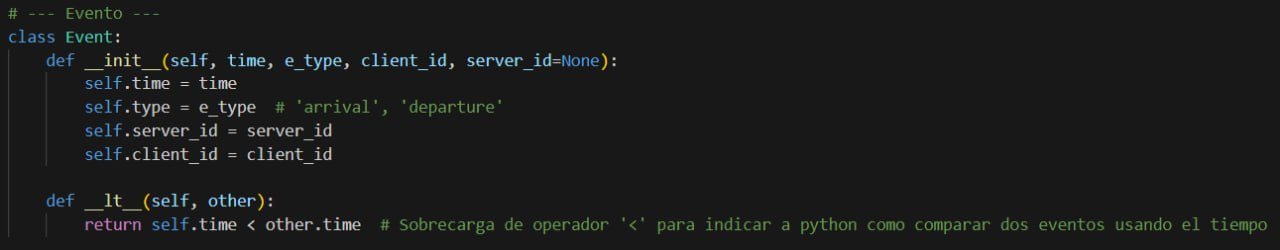
\includegraphics[width=1\textwidth]{event.jpg}
\end{figure}

\newpage
Esta clase se encarga de gestionar y contener la información necesaria para cada evento. Dichos eventos tienen
dos tipos:
\begin{itemize}
\item Eventos de llegada: Contienen un tiempo, el tipo 'arrival' y el ID del cliente que llega.
\item Eventos de salida: Contienen un tiempo, el tipo 'departure', el ID del cliente que sale y el ID del servidor del cual se sale.
\end{itemize}
También se cuenta con el método genérico de la simulación 'simulate\_queueing\_system' que recibe como parámetros la cantidad de servidores en paralelo, la tasa de llegada de clientes, las tasas de atención para cada servidor y el límite de tiempo durante el cual debe correr la simulación, y su salida contiene el promedio de tiempo de los clientes en el sistema, el promedio de tiempo de espera en cola de los clientes, el tiempo total de procesamiento de cada servidor, los tiempos de llegada y salida de cada cliente y la cantidad de clientes atendidos por cada servidor.

\subsection{Lógica de la simulación}
La función 'simulate\_queueing\_system' tras inicializar todas sus listas y variables, genera un primer evento de llegada y comienza
su procesamiento. Los eventos se ordenan según el tiempo debido a la definición previamente realizada en la clase Event en conjunto
con el sistema de heap en que se contienen los eventos. Para cada evento analizado, se verifica su tipo y se ejecuta un
procedimiento que puede ser la inserción de un nuevo ciente a un servidor, a la cola de espera o dar salida a un cliente. Durante
este proceso se van guardando tiempos y variables de importancia y finalmente se generan más llegadas de clientes. Al finalizar
el tiempo límite no existe garantía de que todos los clientes en cola hayan sido debidamente procesados, lo cual simula un sistema
de colas real con cumplimiento estricto de horario.

\subsection{Ejecuciones de pruebas realizadas}
Se realizaron numerosas pruebas a partir de esta simulación, cada una con un aspecto importante que medir y varios parámetros de
entrada modificados. Generalmente, y para mejor entendimiento, estas pruebas varían un parámetro a la vez y generan un gráfico
comparativo que incluye medidas de tendencia central como punto representativo en cada simulación realizada, y son realizadas
varias simulaciones para cada objetivo a comprobar para mejorar la estabilidad y consistencia de la observación realizada.
Estas pruebas están enumeradas y contienen una breve descripción del objetivo que se busca comprobar y a qué modificaciones está
sujeta la entrada de la simulación.

\section{Resultados y experimentos}
\subsection{Hallazgos de la simulación}
Tras la realización de los experimentos, se ha podido llegar a las siguientes conclusiones:
\begin{itemize}
\item Al aumentar el número de servidores, disminuye considerablemente el promedio de tiempo de espera de los clientes en la cola. Sin embargo, de un cierto número en adelante se considera innecesario seguir aumentando el número de servidores ya que el tiempo de espera promedio es cero.
\item Al trabajar con dos servidores en igualdad de condiciones y una tasa de llegada media, se distribuye casi equitativamente el entre servidores. Pero al aumentar la tasa de servicio de uno de ellos, el sistema asigna significativamente más clientes a este servidor. También se ha notado que como existe una estrategia no equitativa de asignación de servidores, siendo de preferencia el servidor con menor ID, los primeros servidores realizan más trabajos que los últimos. 
\item Al aumentar la tasa de llegada de clientes al sistema, aumenta también el tiempo promedio de espera y el tiempo promedio en el sistema de los clientes, debido a que en estos casos la cola se va congestionando poco a poco y los servidores pasan a estar ocupados casi todo el tiempo.
\item En sistemas con tasa de llegada baja de clientes, debido a la preferencia de servidores por orden de ID, los primeros servidores realizan significativamente más trabajo que los últimos. Sin embargo, en colas congestionadas con altas tasas de llegada, el trabajo se distribuye más equitativamente entre todos los servidores.
\item En simulaciones de menor tiempo de duración, los tiempos de espera en cola y tiempos en el sistema de los clientes poseen muchas fluctuaciones, dando a indicar la presencia de cuellos de botella durante breves congestiones del sistema. Sin embargo, un tiempo más largo de duración tiende a estabilizar estas medidas.
\item Al trabajar en colas congestionadas, dos servidores en igualdad de condiciones pasan casi el mismo tiempo de funcionamiento. Si aumentamos la tasa de procesamiento de uno de los servidores, el resultado es prácticamente el mismo. Sin embargo, si en vez de medir el  tiempo de funcionamiento medimos la carga de trabajo, un servidor realiza significativamente más proceso que el otro, aunque demoren más o menos el mismo tiempo de trabajo.
\item Si medimos el tiempo de entrada y salida de cada cliente en una cola con baja tasa de llegada y alta tasa de procesamiento de los servidores, pocos o ningún cliente dejan de ser atendidos. Mientras más grande sea la tasa de llegada y menor sea la tasa de  procesamiento de los servidores, más clientes dejarán de ser atendidos y permanecerán en la cola de espera al finalizar el tiempo.
\end{itemize}

\subsection{Interpretación de los resultados}
Podemos interpretar los resultados de la simulación de la siguiente manera:
\begin{itemize}
\item Relación entre número de servidores y tiempos de espera: Se evidencia que incrementar el número de servidores reduce  significativamente el tiempo de espera en cola. Sin embargo, una vez que se alcanza un punto en el que los clientes son atendidos de forma inmediata (tiempo de espera promedio cercano a cero), añadir más servidores resulta redundante y no contribuye a una  mejora significativa en el rendimiento del sistema.
\item Distribución del trabajo entre servidores: Cuando todos los servidores tienen la misma capacidad de servicio, el sistema  distribuye casi equitativamente las solicitudes. No obstante, al introducir servidores con mayor tasa de servicio, estos son  preferidos por el sistema, absorbiendo una mayor carga de trabajo. Además, la estrategia de asignación por orden de ID  (preferencia por el primer servidor disponible) provoca que los servidores con ID más bajo procesen más clientes, especialmente en condiciones de baja congestión.
\item Impacto de la tasa de llegada: Un aumento en la tasa de llegada genera congestión en el sistema, incrementando tanto los tiempos de espera como el tiempo total que los clientes pasan en el sistema. Esto demuestra la sensibilidad del sistema a la relación entre la tasa de llegada y la tasa de servicio, siendo crucial balancear ambos parámetros para evitar cuellos de botella.
\item Efecto del tiempo de simulación: Simulaciones de corta duración presentan una mayor variabilidad en los resultados, como tiempos de espera irregulares y distribución desigual de carga entre servidores, debido a que el sistema aún no alcanza un estado  estacionario. Simulaciones más largas tienden a estabilizar las métricas, proporcionando una visión más confiable del  comportamiento promedio del sistema.
\item Medición de carga vs. tiempo de uso: Aunque dos servidores puedan estar activos durante lapsos similares, la cantidad de trabajo procesado (es decir, la carga total) puede diferir significativamente si uno de ellos posee una tasa de servicio más alta.  Esto resalta la importancia de considerar no solo el tiempo activo de los servidores, sino también su capacidad efectiva para  comparar eficiencia.
\item Atención completa vs. clientes no atendidos: En escenarios con baja tasa de llegada y alta capacidad de servicio, prácticamente  todos los clientes son atendidos durante la simulación. En contraste, una tasa de llegada superior a la capacidad del sistema  provoca acumulación de clientes en la cola y deja solicitudes pendientes al finalizar la simulación, lo que representa una  pérdida de eficiencia y satisfacción del cliente.
\end{itemize}

\subsection{Hipótesis extraídas de los resultados}
\begin{itemize}
\item H1: A partir de un cierto número de servidores, agregar más servidores no reduce significativamente el tiempo promedio de espera.
\item H2: El sistema tiende a asignar más clientes a los servidores con menor identificador.
\item H3: En condiciones de alta congestión (alta tasa de llegada), la carga de trabajo se distribuye más equitativamente entre todos 
los servidores.
\item H4: Al aumentar la tasa de llegada, el tiempo promedio en el sistema de los clientes también aumenta.
\item H5: En sistemas con servidores de diferentes capacidades, los servidores con mayor tasa de servicio tienden a procesar más 
clientes, incluso si operan durante el mismo período de tiempo.
\item H6: En simulaciones de mayor duración, las métricas de rendimiento del sistema tienden a estabilizarse.
\item H7: Si la tasa de llegada supera la capacidad conjunta de servicio, un número creciente de clientes quedará sin ser atendido 
al final de la simulación.
\end{itemize}

\newpage
\subsection{Experimentos realizados para validar las hipótesis}
\textbf{Validación de H1}: Se ejecutaron simulaciones variando el número de servidores (2, 3 y 5) manteniendo constante la tasa
de llegada y las tasas de servicio.\\
\begin{figure}[!!h]
    \centering
    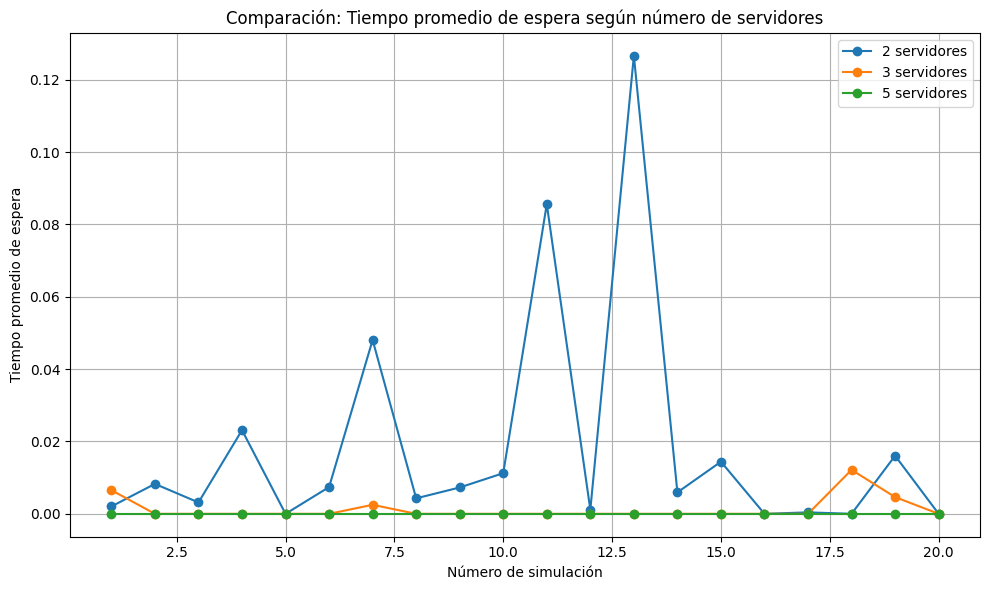
\includegraphics[width=1\textwidth]{Server_ammount_comparisson.png}
\end{figure}\\\vspace{0.2cm}
Conclusiones: \\
A partir de cierto número (probablemente 4 o 5), el tiempo promedio de espera en cola se estabiliza en cero
o cerca de cero.\\\vspace{1cm}

\textbf{Validación de H2}: Se simuló el sistema con dos servidores con una misma tasa de servicio en diferentes lapsos de tiempo.
La tasa de llegada de clientes era considerablemente baja.\\
\begin{figure}[!!h]
    \centering
    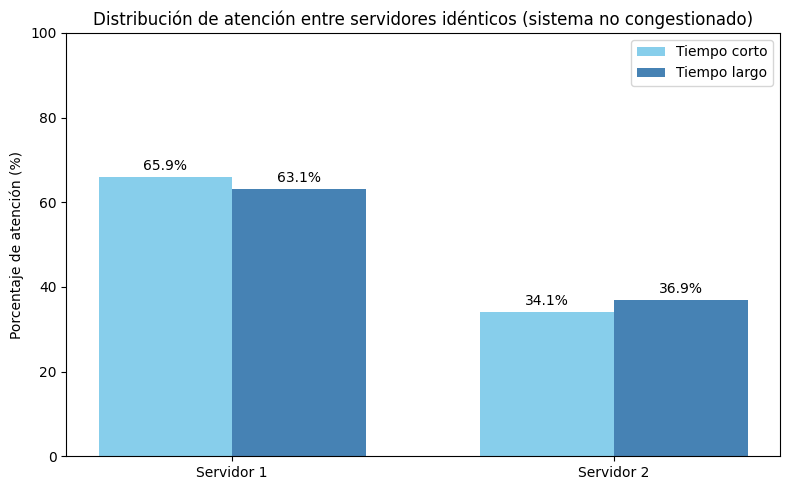
\includegraphics[width=0.6\textwidth]{No_congestion_attention_comparisson.png}
\end{figure}\\\vspace{0.2cm}
\newpage
Conclusiones: El primer servidor (ID más bajo) procesó consistentemente más clientes que los últimos en ambos casos. La política
de asignación favorece al primer servidor libre, lo que genera una carga desequilibrada cuando la cola no está saturada.\\\vspace{1cm}

\textbf{Validación de H3}: Se simuló el sistema con dos servidores con una misma tasa de servicio en diferentes lapsos de tiempo.
La tasa de llegada de clientes era bastante alta.\\
\begin{figure}[!!h]
    \centering
    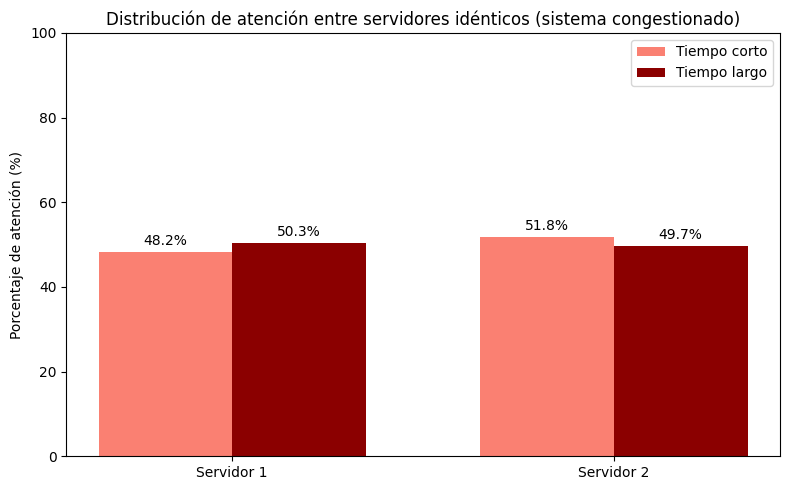
\includegraphics[width=0.6\textwidth]{Congestion_attention_comparisson.png}
\end{figure}
Conclusiones: Cuando todos los servidores están ocupados constantemente, las decisiones de asignación se ven forzadas a usar 
todos los recursos disponibles. A medida que la cola se congestiona, los servidores más rezagados comienzan a participar más
en el procesamiento, y la diferencia de carga entre servidores disminuye.\\\vspace{1cm}

\textbf{Validación de H4}: Se compararon simulaciones con diferentes tasas de llegada, dejando constantes el número de servidores y 
sus tasas de servicio.\\
\begin{figure}[!!h]
    \centering
    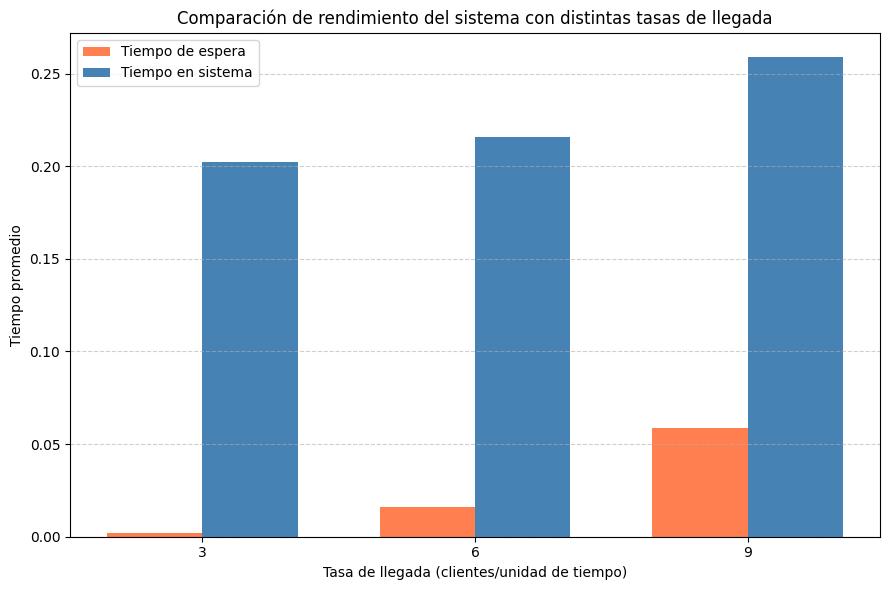
\includegraphics[width=0.6\textwidth]{Arrival_time_rate_comparisson.png}
\end{figure}
Conclusiones: Una mayor tasa de llegada genera acumulación de clientes en la cola, lo que incrementa el tiempo total desde la
llegada hasta la salida. El tiempo promedio de espera y el tiempo total en el sistema aumentan con la tasa de llegada.\\\vspace{1cm}

\textbf{Validación de H5}: Se configuró un sistema con dos servidores, donde en un caso uno tenía mayor tasa de servicio que el otro y en el otro caso ambos tenían la misma tasa.\\
\begin{figure}[!!h]
    \centering
    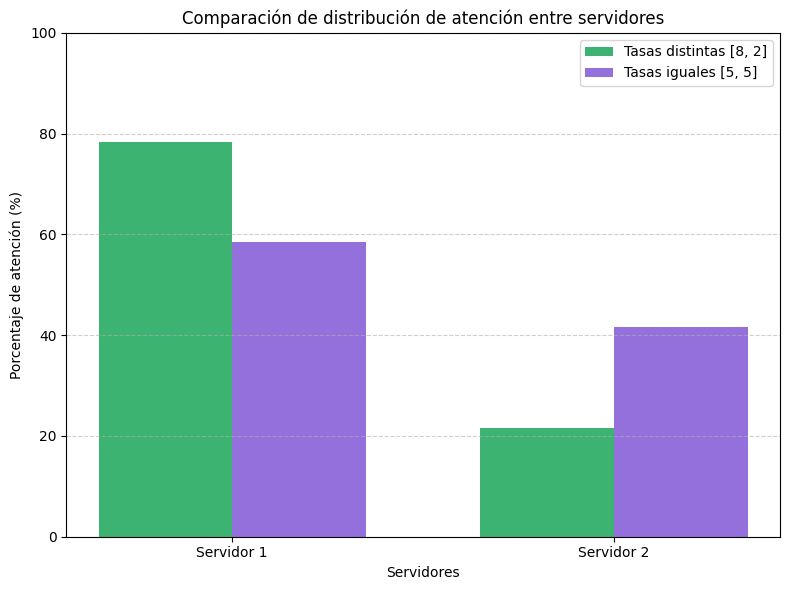
\includegraphics[width=0.6\textwidth]{Service_time_rate_comparisson.png}
\end{figure}
\begin{figure}[!!h]
    \centering
    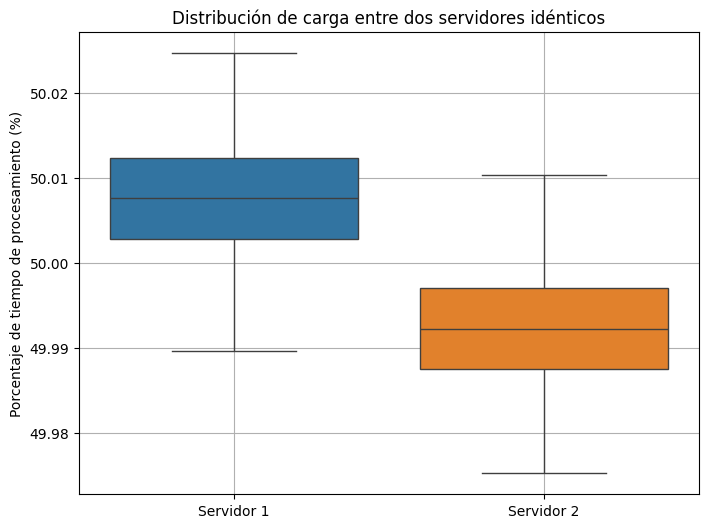
\includegraphics[width=0.6\textwidth]{Congested_processing_time_comparisson.png}
\end{figure}
\begin{figure}[!!h]
    \centering
    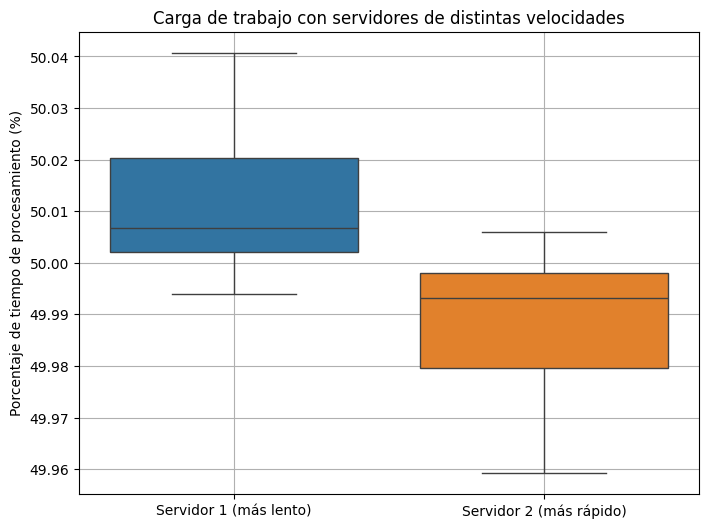
\includegraphics[width=0.5\textwidth]{Different_speed_processing_time_comparisson.png}
\end{figure}
\newpage
Conclusiones: A igual tiempo activo, una mayor velocidad de servicio implica mayor volumen de trabajo realizado. El servidor más
rápido procesó un número significativamente mayor de clientes, aunque ambos permanecieron ocupados casi el mismo tiempo.\\\vspace{1cm}

\textbf{Validación de H6}: Se ejecutaron simulaciones con diferentes duraciones (Caso 1: 500 unidades de tiempo | Caso 2: 10000 unidades de tiempo) y se evaluaron las variaciones del tiempo medio de espera y tiempo medio en el sistema.\\
\begin{figure}[!!h]
    \centering
    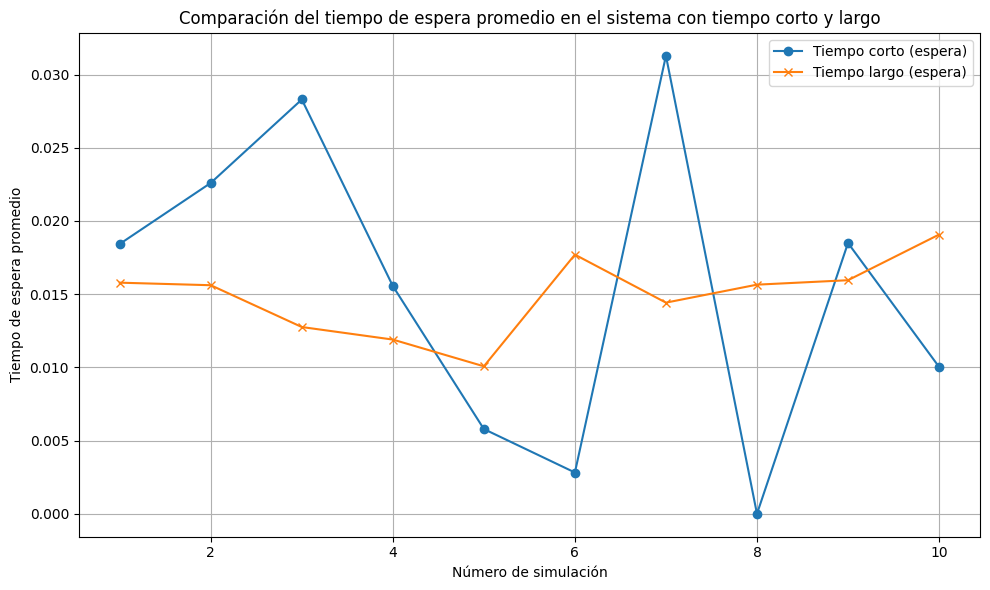
\includegraphics[width=0.6\textwidth]{Variation_of_waiting_time.png}
\end{figure}
\begin{figure}[!!h]
    \centering
    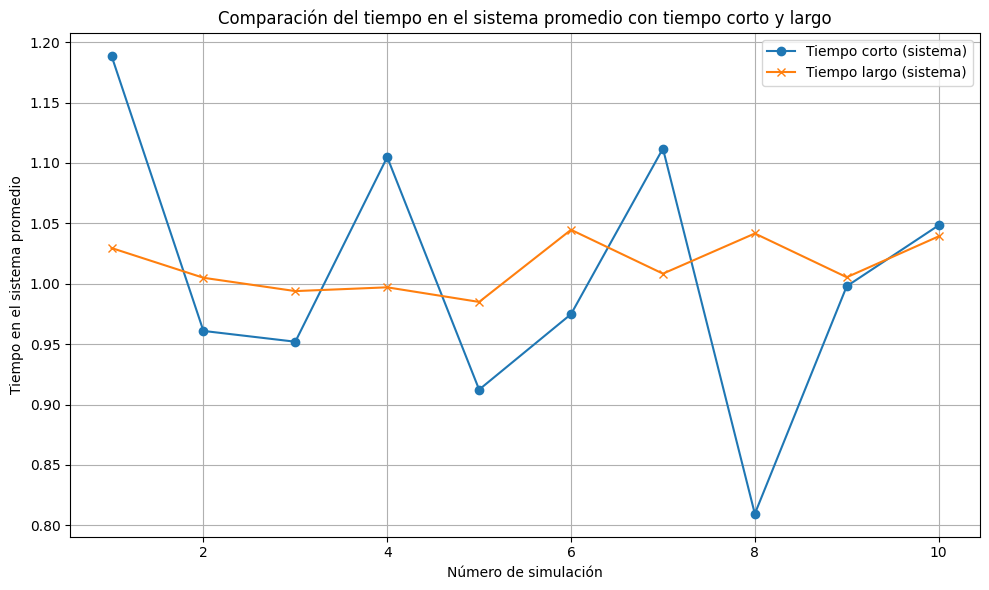
\includegraphics[width=0.6\textwidth]{Variation_of_system_time.png}
\end{figure}
\\Conclusiones: Se observó que en simulaciones cortas hay fluctuaciones significativas, mientras que en simulaciones largas el 
sistema alcanza un estado estacionario.\\\vspace{1cm}

\textbf{Validación de H7}: Se realizaron dos pruebas. En una se aumentó la tasa de llegada mientras que en la otra se disminuyó. Se puso en observación el tiempo de llegada y salida de cada cliente.\\
Conclusiones: El sistema no puede vaciar la cola si entran más clientes por unidad de tiempo de los que se pueden procesar.
En la prueba con alta tasa de llegada quedaban al final una cantidad mayor de clientes sin atender que en la prueba con una
tasa de llegada más baja, manteniendo la igualdad de condiciones de ambos sistemas en los parámetros restantes.\\
\newpage
\begin{figure}[!h]
    \centering
    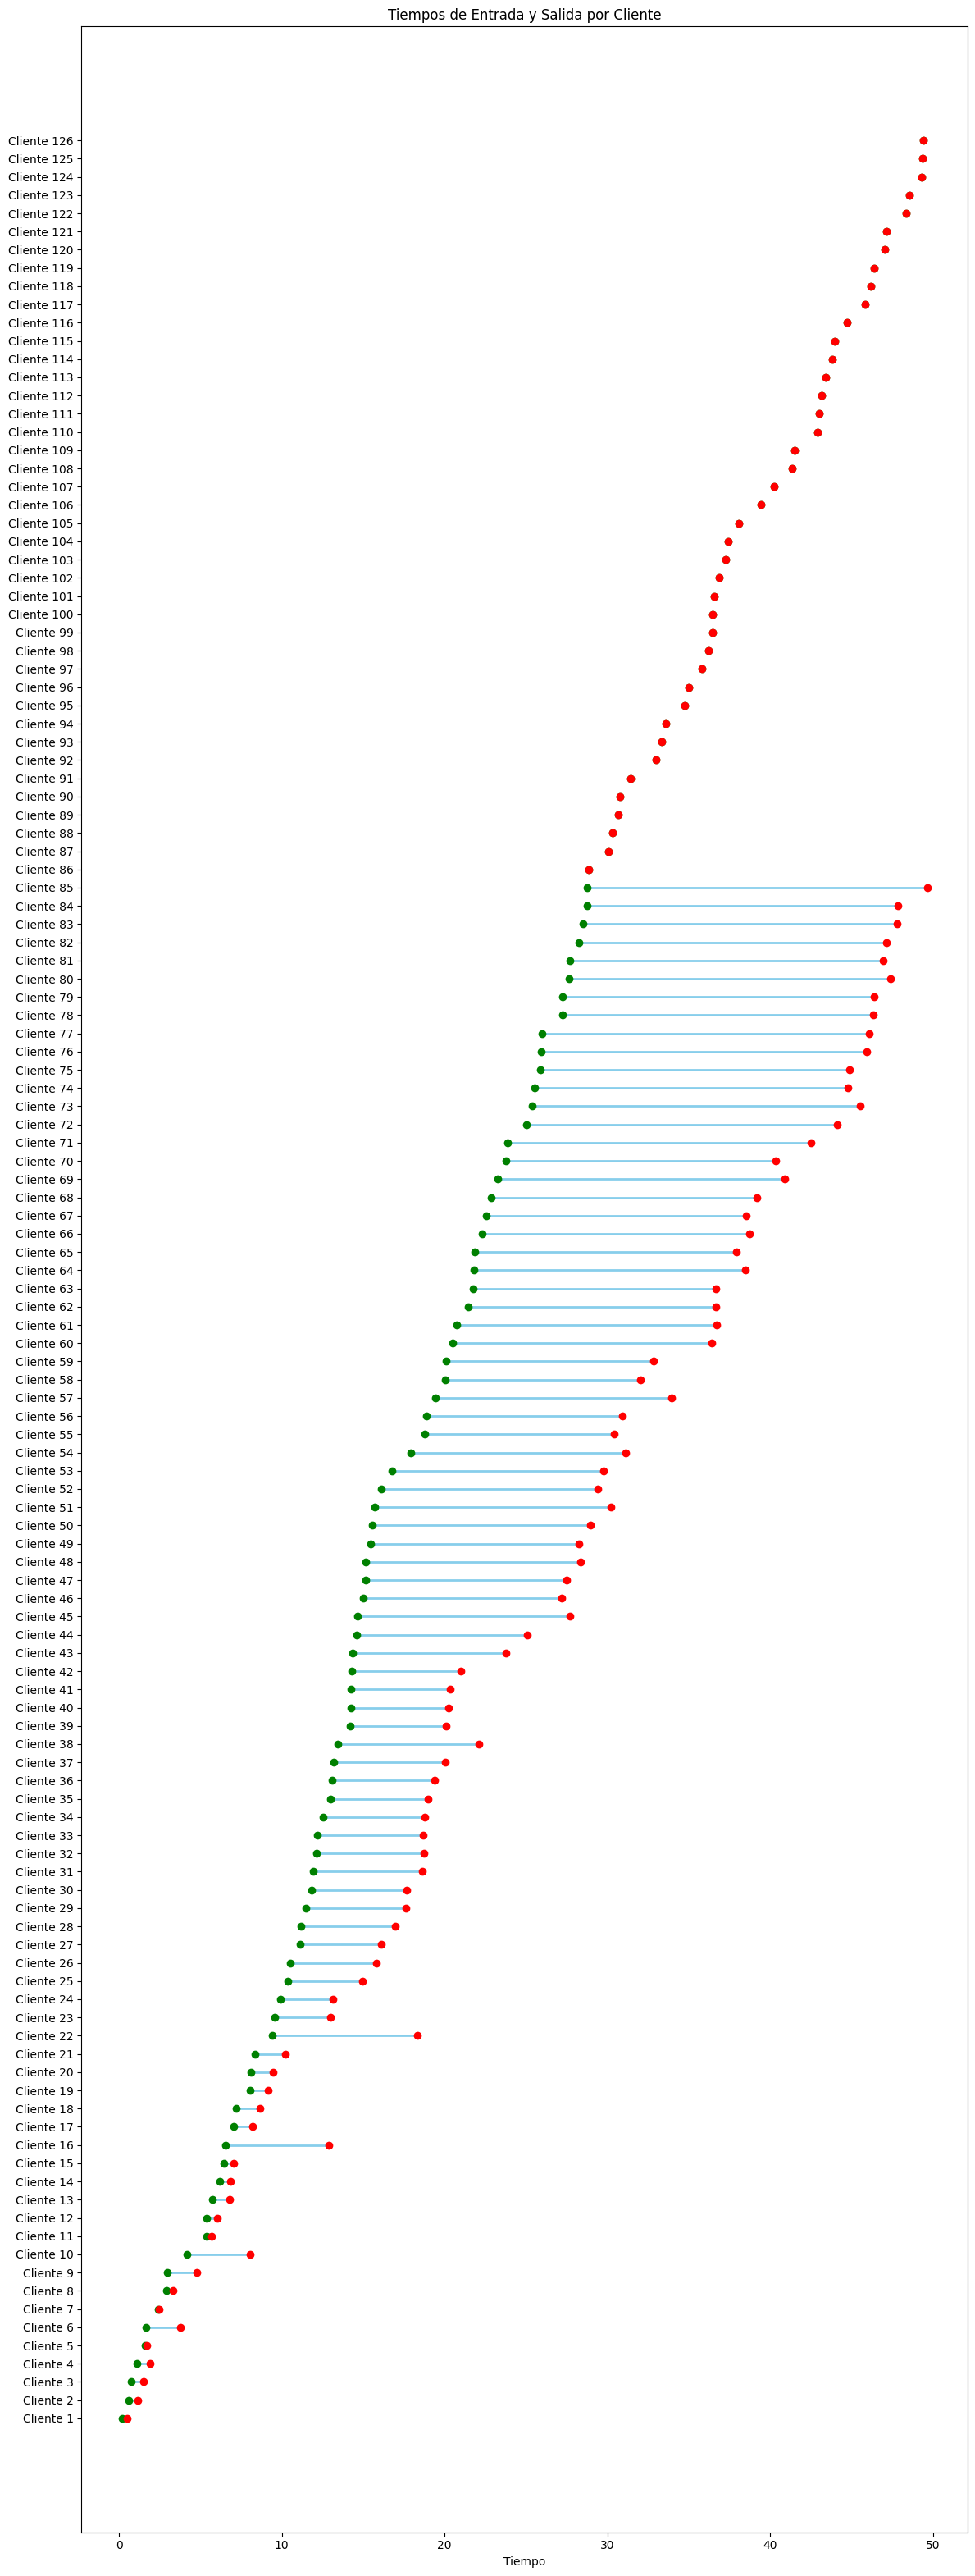
\includegraphics[width=0.5\textwidth]{Congested_queue_time_analisis.png}
\end{figure}
\begin{figure}[!h]
    \centering
    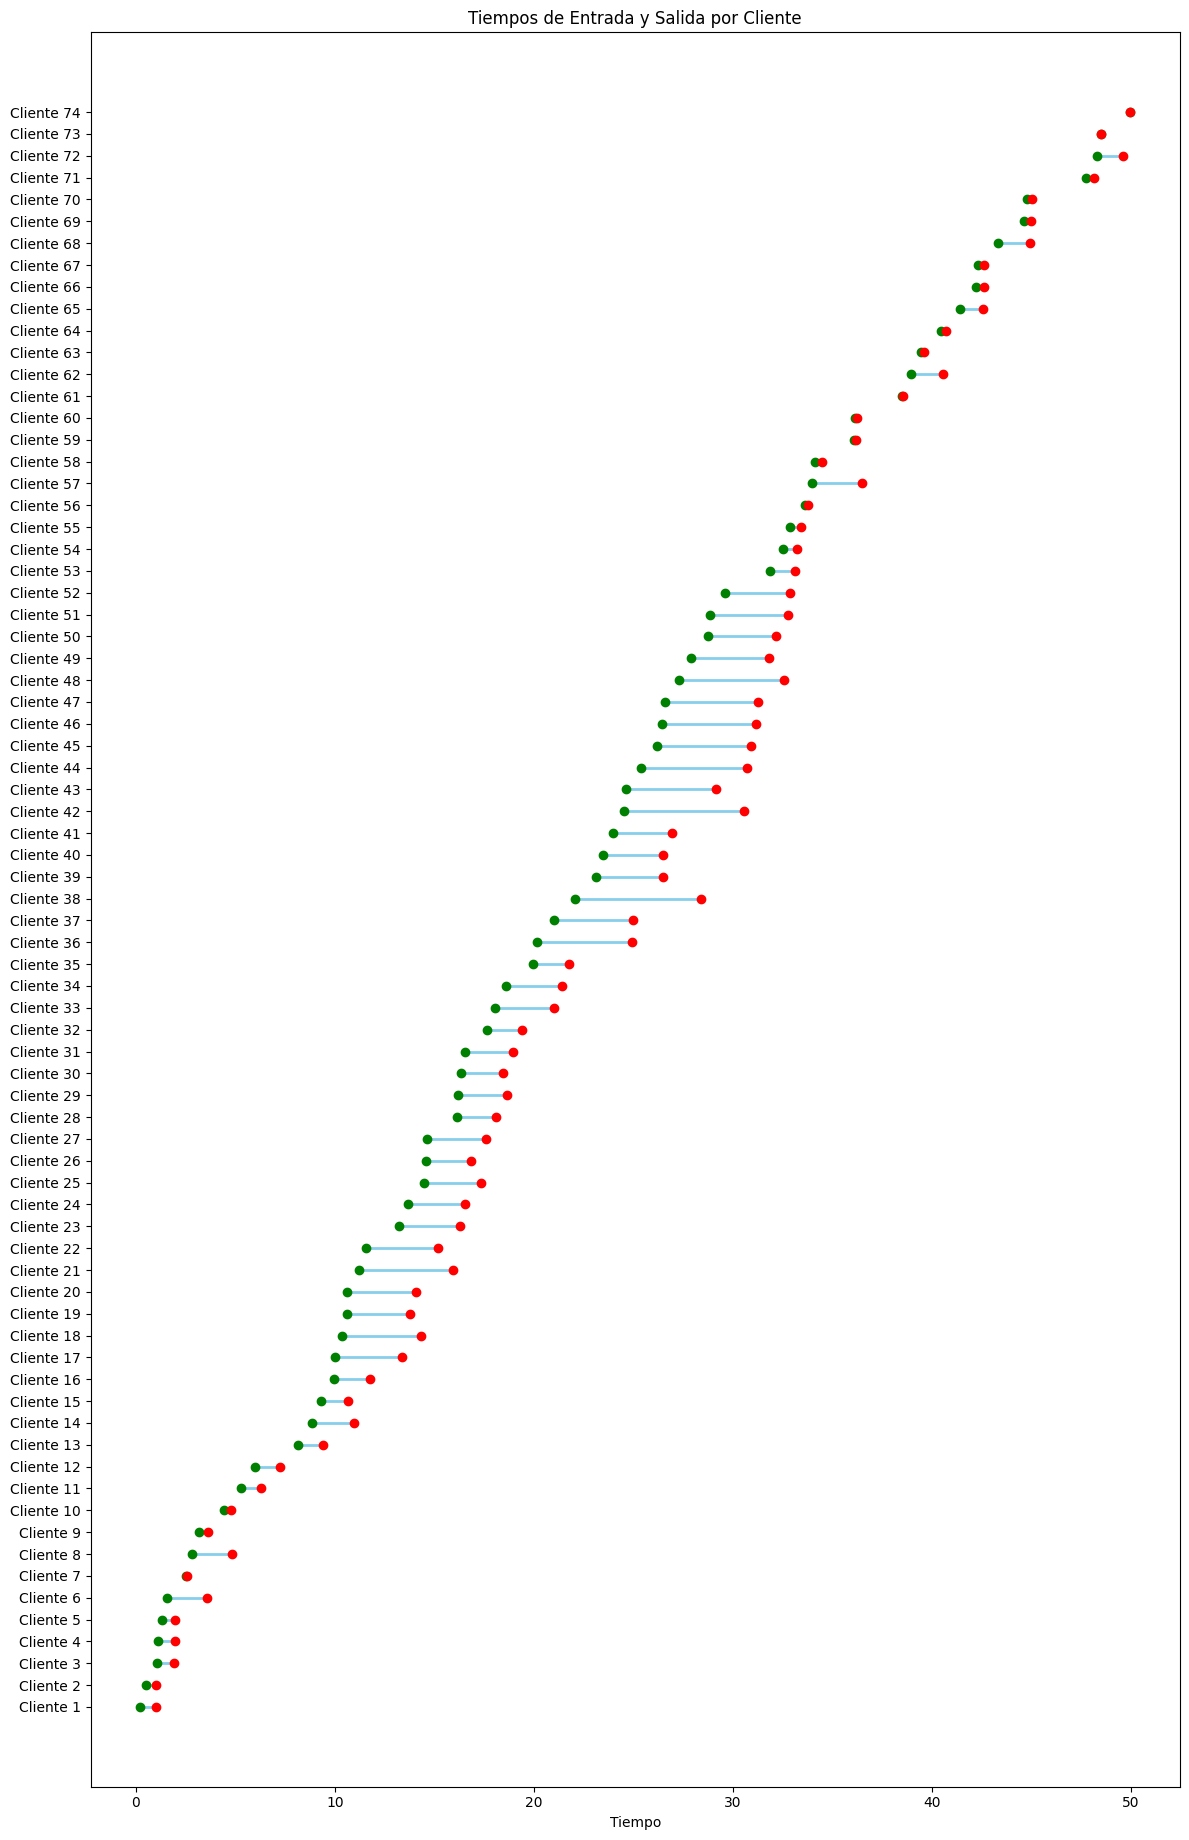
\includegraphics[width=0.5\textwidth]{No_Congested_queue_time_analisis.png}
\end{figure}

\newpage
\newpage
\subsection{Necesidad de realizar el análisis estadístico de la simulación (Variables de interés)}
Es necesario comprobar estadísticamente si nuestras hipótesis son correctas, pues a pesar de que se realizan varias ejecuciones
por prueba, debemos descartar cualquier posible fallo. Por tanto, cada una de las 7 hipótesis extraídas del análisis tiene
sus propias comprobaciones (archivo stats\_validator.ipynb) como se describe a continuación:\\
\begin{itemize}
\item \textbf{Hipótesis 1}: Se realizó una prueba t de Student para comparar los promedios de tiempo de espera de varios grupos con diferentes cantidades de servidores. La prueba consiste en comparar medias de dos grupos: aquellos con altos promedios de tiempo con los que tienen promedio cero. La prueba resultó exitosa y respaldó H1. Las variables de interés analizadas son:
\begin{itemize}
\item Lista de número de servidores de cada ejecución
\item Tiempo promedio de espera de cada ejecución
\end{itemize}
\item \textbf{Hipótesis 2}: Se usó una prueba de Chi-cuadrado para comparar la distribución observada de clientes por servidor contra una distribución uniforme esperada (si todos fueran asignados de forma equitativa). Se comprobó que la asignación no es equitativa,
con una preferencia por servidores de menor ID, por lo cual H2 queda respaldada. Las variables de interés analizadas son:
\begin{itemize}
\item Lista con cantidad de clientes atendidos por cada servidor
\end{itemize}
\item \textbf{Hipótesis 3}: Comparamos la varianza en la carga de trabajo entre los servidores en distintos niveles de congestión  (diferentes tasas de llegada).\\
Si la varianza disminuye a medida que aumenta la congestión, es señal de una distribución más
equitativa. \\
Con ANOVA verificamos si hay diferencias significativas entre la distribución de cargas en distintos escenarios de congestión. Tras ejecutar la comprobación, queda respaldada la hipótesis 3. Las variables de interés analizadas son:
\begin{itemize}
\item Lista con cantidad de clientes atendidos por cada servidor
\item Distribución de llegada de cada comprobación
\end{itemize}
\item \textbf{Hipótesis 4}: Se usará una regresión lineal simple, ya que queremos ver si hay una relación lineal positiva entre:
\begin{itemize}
\item Variable independiente: Tasa de llegada.
\item Variable dependiente: Tiempo promedio en el sistema.
\end{itemize}
Si la pendiente (slope) es positiva y el p-valor es menor que 0.05, entonces podemos decir que existe una relación significativa:
a mayor tasa de llegada, mayor tiempo en el sistema. El resultado respalda H4 debido a que existe una relación lineal positiva
entre las variables anteriores.
\item \textbf{Hipótesis 5}: Se busca comprobar si los servidores con mayor tasa de servicio (mayor velocidad) atienden más clientes. Para esto se usará regresión lineal simple para comprobar si existe una relación significativa entre:
\begin{itemize}
\item Variable independiente (X): tasa de servicio de cada servidor
\item Variable dependiente (Y): cantidad de clientes atendidos por cada servidor
\end{itemize}
El resultado respalda H5 debido a que existe una relación lineal positiva entre las variables anteriores.
\item \textbf{Hipótesis 6}:  Se comprobó si, al aumentar la duración de la simulación, la variabilidad disminuye, lo que indicaría que las métricas se estabilizan con el tiempo. Se aplicó la prueba coeficiente de correlación de Spearman entre:
\begin{itemize}
\item Duración de la simulación
\item Desviación estándar del tiempo de espera
\end{itemize}
Si hay una correlación negativa significativa, se valida la hipótesis: a mayor duración, menor variabilidad. El resultado
concluyó que no se puede validar H6 debido a que no existe una evidencia significativa de estabilización, pues la desviación
estándar sigue creciendo aunque aumente el tiempo de simulación. POR TANTO, ESTA HIPÓTESIS QUEDA DESCARTADA.
\item \textbf{Hipótesis 7}:  Se comprobó si, al aumentar la tasa de llegada, también aumenta la cantidad de clientes sin atender. Se aplicó la prueba coeficiente de correlación de Spearman entre:
\begin{itemize}
\item Tasa de llegada
\item Número de clientes sin atender
\end{itemize}
Si hay una correlación positiva y significativa valida la hipótesis: a más llegadas, más clientes no atendidos. El resultado concluyó que se valida H7 debido a la existencia de esta correlación.
\end{itemize}

\subsection{Análisis de parada de la simulación}
Para garantizar que los resultados obtenidos en la simulación sean representativos del comportamiento estable del sistema,
se realizó un análisis de parada, evaluando cómo varían las métricas clave (como el tiempo de espera promedio) en función de
la duración de la simulación. Para estabilizar los resultados, se fijó un valor de 10000 unidades de tiempo a análisis que
requieran tiempos largos de ejecución, un valor de 500 unidades de tiempo para análisis que requieran tiempos cortos de
ejecución y un valor de 50 para análisis que requieran un tiempo extremadamente corto de ejecución. El valor más usado fue
el de tiempos largos. Bajo esta configuración controlada, se consiguió un muestreo representativo del funcionamiento del
modelo en cada una de las pruebas realizadas.

\section{Modelo matemático}
\subsection{Descripción del modelo como modelo probabilístico}
El sistema se modela como un proceso estocástico de eventos discretos en tiempo continuo, compuesto por dos flujos aleatorios
principales: el de llegadas de clientes y el de servicios por parte de los servidores. Este modelo es conocido como M/M/c, donde:
\begin{itemize}
\item M (Markovian) en las llegadas: los tiempos entre llegadas siguen una distribución exponencial con una tasa $\lambda$.
\item M (Markovian) en los servicios: los tiempos de proceso en cada servidor también siguen una distribución exponencial, con tasa µ.
\item c: el número de servidores en paralelo.
\end{itemize}

\subsection{Supuestos y restricciones}
Los supuestos y restricciones que describen esta variación particular del modelo son las siguientes:
\begin{itemize}
\item Los tiempos entre llegadas siguen una distribución exponencial con una tasa $\lambda$.
\item Los tiempos de proceso en cada servidor también siguen una distribución exponencial, con tasa µ.
\item El orden de atención es por llegada FCFS (First Come, First Served).
\item No hay límite de tamaño de cola.
\item Una vez que un cliente es insertado en la cola o en un servidor, no puede abandonar el sistema hasta
culminar el proceso.
\item Los servidores no fallan ni se interrumpen.
\item Todos los clientes son tratados de forma homogénea (sin preferencias)
\item No hay tiempo de setup entre servicios
\item La asignación de clientes a servidores es prioritaria por orden de ID (el servidor libre con ID más bajo atiende primero).
\end{itemize}

\subsection{Comparación de los resultados obtenidos con los resultados experimentales}
De las 7 hipótesis que pudimos extraer de los resultados obtenidos, todas excepto H6 resultaron validadas por diversas
pruebas estadísticas como Chi-cuadrado, regresión lineal, ANOVA y Spearman. La presente comparación mostrará los resultados
esperados según el modelo, contra estas validaciones:
\begin{itemize}
\item H1 fue validada: La comparación de medias mostró la diferencia significativa entre servidores. Por otro lado, el modelo muestra
que a partir de cierto punto, agregar más servidores no mejora significativamente el rendimiento. Por tanto, esto representa una
coincidencia con el modelo.
\item H2 fue validada: Chi-cuadrado mostró una distribución no uniforme. Sin embargo, el modelo no especifica una política de 
asignación, aunque se asume balanceo. En este caso la asignación por ID rompe la equidad. Por tanto, no es simétrico en este
aspecto con el modelo estándar M/M/c.
\item H3 fue validada: ANOVA no mostró diferencias significativas en cargas con alta congestión. Luego, El modelo M/M/c asume 
asignación aleatoria inmediata a cualquier servidor libre, lo que favorece balanceo en condiciones de alta carga. Esto 
representa otra coincidencia con el modelo estándar.
\item H4 fue validada: La regresión lineal fue positiva, y M/M/c predice que si $\lambda$ aumenta y µ$*c$ se mantiene constante, $W$ y $W_q$ aumentan. Por tanto, esto representa otra coincidencia con el modelo.
\item H5 fue validada: El test de medias realizado estableció que para datos suficientemente grandes, existe una relación positiva
entre tasas de servicio de servidores y clientes procesados. En M/M/c heterogéneo (distintas tasas de servicio), los más rápidos
absorben más carga si no hay balance explícito. Esto representa otra coincidencia con el modelo.
\item H6 no fue validada: La teoría dice que con simulaciones más largas, las métricas deberían converger (Ley de los grandes números).
Pese a esto, no pudimos validar la hipótesis con los datos simulados. Esto puede deberse a una duración insuficiente o presencia 
de tendencia en el modelo simulado.
\item H7 fue validada: Spearman confirmó la relación positiva entre $\lambda$ y la cantidad de clientes no atendidos. Luego, M/M/c predice congestión creciente si $\rho>1$. Por tanto esto también resulta en una coincidencia con el modelo estándar.
\end{itemize}

\section{Conclusiones}
De las siete hipótesis propuestas para estudiar el comportamiento del sistema de colas con múltiples servidores, seis fueron
validadas estadísticamente mediante pruebas como t de Student, ANOVA, Chi-cuadrado y correlación de Spearman. Se confirma que agregar servidores reduce el tiempo de espera, aunque más allá de cierto punto, no aporta mejoras significativas (H1). La estrategia de asignación por menor identificador genera una distribución desigual del trabajo (H2). En contextos de alta congestión, la carga se reparte más equitativamente entre los servidores (H3). A mayor tasa de llegada, aumenta el tiempo promedio que los clientes pasan en el sistema (H4). Los servidores más rápidos atienden más clientes, incluso si todos están activos el mismo tiempo (H5). Al aumentar la tasa de llegada más allá de la capacidad conjunta, más clientes quedan sin ser atendidos (H7). La hipótesis H6, que planteaba que las métricas se estabilizan al aumentar el tiempo de simulación, no pudo validarse estadísticamente, aunque mostró tendencias consistentes. Al comparar los resultados simulados con las fórmulas teóricasdel modelo M/M/c, se observa una coincidencia cualitativa en tendencias como la reducción del tiempo de espera con más servidores,el impacto del nivel de utilización $\rho$, y el crecimiento del tiempo en cola con alta carga. Sin embargo, debido a elementos no ideales (como la asignación no equitativa de clientes y la variabilidad estocástica), los resultados simulados presentan desviaciones respecto a los valores exactos del modelo teórico.\\
Las pruebas estadísticas han permitido validar o refutar hipótesis con rigor, más allá de simples observaciones visuales o suposiciones. Estas pruebas fueron esenciales para detectar tendencias significativas y evitar conclusiones erróneas en base a datos ruidosos o muestras pequeñas.\\
La simulación desarrollada ha demostrado ser efectiva para modelar sistemas de colas con múltiples servidores y condiciones variables. Los resultados obtenidos refuerzan el conocimiento teórico sobre modelos M/M/c, mientras que las validaciones estadísticas aportan robustez y credibilidad a las conclusiones del estudio.

\section{Bibliografía y referencias}
\begin{itemize}
\item Ross, S. M. (2012). Simulation, Fifth Edition (Epígrafe 7.4: A Queueing System with Two Parallel Servers)
\item Luciano García Garrido. Temas de Simulación.
\end{itemize}

\end{document}